\chapter{Semantic Modeling}
What would you call a world in which any number of people can speak,
when you never know who has something useful to say, and when someone
new might come along at any time and make a valuable but unexpected
contribution? What if just about everyone had the same goal of advancing
the collaborative state of knowledge of the group, but there was little
agreement (at first, anyway) about how to achieve it?

If your answer is ``That sounds like the Web and Semantic Web!'', you
are right (and you must have read Chapter~\ref{ch1}). If your answer is ``It
sounds like any large group trying to understand a complex phenomenon,''
you are even more right. The jungle that is the Semantic Web is not a
new thing; this sort of chaos has existed since people first tried to
make sense of the world around them.

What intellectual tools have been successful in helping people sort
through this sort of tangle? Any number of analytical tools has been
developed over the years, but they all have one thing in common: They
help people understand their world by forming an abstract description
that hides certain details while illuminating others. These abstractions
are called models, and they can take many forms.

How do models help people assemble their knowledge? Models assist in
three essential ways:


\begin{enumerate}
\def\labelenumi{\arabic{enumi}.}
\item
  \emph{Models help people communicate}. A model describes the situation
  in a particular way that other people can understand.
\item
  \emph{Models explain and make predictions}. A model relates primitive
  phenomena to one another and to more complex phenomena, providing
  explanations and predictions about the world.
\item
  \emph{Models mediate among multiple viewpoints}. No two people agree
  completely on what they want to know about a phenomenon; models
  represent their commonalities while allowing them to explore their
  differences.
\end{enumerate}

The Semantic Web standards have been created not only as a medium in
which people can collaborate by sharing information but also as a medium
in which people can collaborate on models. Models that they can use to
organize the information that they share. Models that they can use to
advance the common collection of knowledge.

How can a model help us find our way through the mess that is the Web?
How do these three features help? The first feature, human
communication, allows people to collaborate on their under- standing. If
someone else has faced the same challenge that you face today, perhaps
you can learn from their experience and apply it to yours. There are a
number of examples of this in the Web today, of newsgroups, mailing
lists, forums, social medias and wikis where people can ask questions
and get answers. In the case in which the information needs are fairly
uniform, it is not uncommon for a community or a company to assemble a
set of ``Frequently Asked Questions,'' or FAQs, that gather the
appropriate knowledge as answers to these questions. As the number of
questions becomes unmanageable, it is not uncommon to group them by
topic, by task, by affected subsystem, and so forth. This sort of
activity, by which information is organized for the purpose of sharing,
is the simplest and most common kind of modeling, with the sole aim of
helping a group of people collaborate in their effort to sort through a
complex set of knowledge.

The second feature, explanation and prediction, helps individuals make
their own judgments based on information they receive. FAQs are useful
when there is a single authority that can give clear answers to a
question, as is the case for technical assistance for using some
appliance or service. But in more interpretive situations, someone might
want or need to draw a conclusion for themselves. In such a situation, a
simple answer as given in a FAQ is not sufficient. Politics is a common
example from everyday life. Politicians in debate do not tell people how
to vote, but they try to convince them to vote in one way or another.
Part of that convincing is done by explaining their position and
allowing the individual to evaluate whether that explanation holds true
to their own beliefs about the world. They also typically make
predictions: If we follow this course of action, then a particular
outcome will follow. Of course, a lot more goes into political
persuasion than the argument, but explanation and prediction are key
elements of a persuasive argument.

Finally, the third feature, mediation of multiple viewpoints, is
essential to fostering understanding in a web environment. As the web of
opinions and facts grows, many people will say things that disagree
slightly or even outright contradict what others are saying. Anyone who
wants to make their way through this will have to be able to sort out
different opinions, representing what they have in common as well as the
ways in which they differ. This is one of the most essential organizing
principles of a large, heterogeneous knowledge set, and it is one of the
major contributions that modeling makes to helping people organize what
they know.

Astrologers and the IAU agree on the planethood of Mercury, Venus,
Earth, Mars, Jupiter, Saturn,

Uranus, and Neptune. The IAU also agrees with astrologers that Pluto is
a planet, but it disagrees by calling it a dwarf planet. Astrologers (or
classical astronomers) do not accept the concept of dwarf planets, so
they are not in agreement with the IAU, which categorizes UB313 and
Ceres as such. A model for the Semantic Web must be able to organize
this sort of variation, and much more, in a meaningful and manageable
way.

\section{Modeling for Human Communication}

Models used for human communication have a great advantage over models
that are intended for use by computers; they can take advantage of the
human capacity to interpret signs to give them meaning. This means that
communication models can be written in a wide variety of forms,
including plain language or ad hoc images. A model can be explained by
one person, amended by another, interpreted

by a third person, and so on. Models written in natural language have
been used in all manner of intellectual life, including science,
religion, government, and mathematics.

But this advantage is a double-edged sword; when we leave it to humans
to interpret the meaning of a model, we open the door for all manner of
abuse, both intentional and unintentional. Legislation provides a good
example of this. A governing body like a parliament or a legislature
enacts laws that are intended to mediate rights and responsibilities
between various parties. Legislation typically sets up some sort of
model of a situation, perhaps involving money (e.g., interest caps,
taxes); access rights (who can view what information, how can
information be legally protected); personal freedom (how freely can one
travel across borders, when does the government have the right to
restrict a person's movements); or even the structure of government
itself (who can vote and how are those votes counted, how can government
officials be removed from office). These models are painstakingly
written in natural language and agreed on through an elaborate process
(which is also typically modeled in natural language).

It is well known to anyone with even a passing interest in politics that
good legislation is not an easy task and that crafting the words
carefully for a law or statute is very important. The same flexibility
of interpretation that makes natural language models so flexible also
makes it difficult to control how the laws will be interpreted in the
future. When someone else reads the text, they will have their own
background and their own interests that will influence how they
interpret any particular model. Readers of the previous paragraph in the
third edition probably interpreted it very differently from readers of
the first edition only a decade earlier, despite the fact that the text
has not changed at all. This phenomenon is so widespread that most
government systems include a process (usually involving a court
magistrate and possibly a committee of citizens) whereby disputes over
the interpretation of a law or its applicability can be resolved.

When a model relies on particulars of the context of its reader for
interpretation of its meaning, as is the case in legislation, we say
that a model is \emph{informal}. That is, the model lacks a formalism
whereby the meaning of terms in the model can be uniquely defined.

In the hypertext web today, there are informal models that help people
communicate about the organization of the information. It is common for
commerce web sites to organize their wares in catalogs with category
names like ``web-cams,'' ``Oxford shirts,'' and ``Granola.'' In such
cases, the communication is primarily one way; the catalogue designer
wants to communicate to the buyers the information that will help them
find what they want to buy. The interpretation of these words is up to
the buyers. The effectiveness of such a model is measured by the degree
to which this is successful. If enough people interpret the categories
in a way similar enough to the intent of the cataloguer, then they will
find what they want to buy. There will be the occasional discrepancy
like ``Why wasn't that item listed as a \emph{webcam}?'' or ``That's not
granola, that's just plain cereal!'' But as long as the interpretation
is close enough, the model is successful.

A more collaborative style of document modeling comes in the form of
community tagging. A number of web sites have been successful by
allowing users to provide meaningful symbolic descriptions of their
content in the form of \emph{tags}. A tag in this sense is simply a
single word or short phrase that describes some aspect of the content.
Early examples of this sort of tagging system include Flickr for photos
and del.icio.us for Web bookmarks. In more modern systems, we see
``hashtags'' in social media like Twitter, LinkedIn and Facebook playing
a similar role. Users of content organization services like Slideshare
for presentations and YouTube for videos use tags to help other users
find and discover content. The idea of community tagging is that each
individual who provides content will describe it using tags of their own
choosing. If any two people use the same tag, this becomes a common
organizing entity; anyone who is browsing for content can access
information from both contributors under that tag. The tagging
infrastructure shows which tags have been used by many people. Not only
does this help browsers determine what tags to use in a search, but it
also helps content providers to find commonly used tags that they might
want to use to describe new content. Thus, a tagging system will have a
certain self-organizing character, whereby popular tags become more
popular and unpopular tags remain unpopular---something like evolution
by artificial selection of tags. The resulting collection of tags and
their relations is called a \emph{Folksonomy} to reflect the fact this
is a categorization from and by the crowd.

Tagging systems of this sort provide an informal organization to a large
body of heterogeneous information. The organization is informal in the
sense that the interpretation of the tags requires human processing in
the context of the consumer. Just because a tag is popular doesn't mean
that everyone is using it in the same way. In fact, the community
selection process actually selects tags that are used in several
different ways, whether they are compatible or not. As more and more
people provide content, the popular tags saturate with a wide variety of
content, making them less and less useful as discriminators for people
browsing for content. This sort of problem is inherent in information
modeling systems; since there isn't an objective description of the
meaning of a symbol outside the context of the provider and consumer of
the symbol, the communication power of that symbol degrades as it is
used in more and more contexts.

Formality of a model isn't a black-and-white judgment; there can be
degrees of formality. This is clear in legal systems, where it is common
to have several layers of legislation, each one giving objective context
for the next. A contract between two parties is usually governed by some
regional law that provides standard definitions for terms in the
contract. Regional laws are governed by national laws, which provide
constraints and definitions for their terms. National laws have their
own structure, in which a constitution or a body of case law provides a
framework for new decisions and legislation. Even though all these
models are expressed in natural language and fall back on human
interpretation in the long run, they can be more formal than private
agreements that rely almost entirely on the interpretation of the
agreeing parties.

This layering of informal models sometimes results in a modeling style
that is reminiscent of Talmudic scholarship. The content of the Talmud
includes not only the original scripture but also interpretative
comments on the scripture by authoritative sources (classical rabbis).
Their comments have gained such respect that they are traditionally
published along with the original scripture for comment by later rabbis,
whose comments in turn have become part of the intellectual tradition.
The original scripture, along with all the authoritative comments, is
collectively called the Talmud, and it is the basis of a classical
Jewish education to this day.

A similar effect happens with informal models. The original model is
appropriate in some context, but as its use expands beyond that context,
further models are required to provide common context to explicate the
shared meaning. But if this further exposition is also informal, then
there is the risk that its meaning will not be clear, so further
modeling must be done to clarify that. This results in heavily layered
models, in which the meaning of the terms is always subject to further
interpretation. It is the inherent ambiguity of natural language at each
level that makes the next layer of commentary necessary until the degree
of ambiguity is ``good enough'' that no more levels are needed. When it
is possible to choose words that are evocative and have considerable
agreement, this process converges much more quickly.

Human communication, as a goal for modeling, allows it to play a role in
the ongoing collection of human knowledge. The levels of communication
can be quite sophisticated, including the collection of information used
to interpret other information. In this sense, human communication is
the fundamental requirement for building a Semantic Web. It allows
people to contribute to a growing body of knowledge and then draw from
it. But communication is not enough; to empower a web of human
knowledge, the information in a model needs to be organized in such a
way that it can be useful to a wide range of consumers.

\section{Explanation and Prediction}

Models are used to organize human thought in the form of explanations.
When we understand how a phenomenon results from other basic principles,
we gain a number of advantages. Not least is the feeling of confidence
that we have actually understood it; people often claim to ``have a
grasp on'' or ``have their head around'' an idea when they finally
understand it. Explanation plays a major role in this sort of
understanding. Explanation also assists in memory; it is easier to
remember that putting a lid on a flaming pot can quench the flame if one
knows the explanation that fire requires air to burn. Most important for
the context of the Semantic Web, explanation makes it easier to reuse a
model in whole or in part; an explanation relates a conclusion to more
basic principles. Understanding how a pot lid quenches a fire can help
one understand how a candle snuffer works. Interpretability and
explanation are vital for establishing trust in a model and to
effectively support decision making. You are more likely to trust my
model, if I can provide results you can interpret and explanations so
that you can understand why the model is appropriate. Interpretability
and explanation are the keys to understanding when a model is applicable
and when it is not.

Closely related to this aspect of a model is the idea of prediction.
When a model provides an adequate explanation of a phenomenon, it can
also be used to make predictions. This aspect of models is what makes
their use central to the scientific method, where falsification of
predictions made by models forms the basis of the methodology of
inquiry.

Explanation and prediction typically require models with a good deal
more formality than is usually required for human communication. An
explanation relates a phenomenon to ``first principles''; these
principles, and the rules by which they are related, do not depend on
interpretation by the consumer but instead are in some objective form
that stands outside the communication. Such an objective form, and the
rules that govern how it works, is called a formalism.

Formal models are the bread and butter of mathematical modeling, in
which very specific rules for calculation and symbol manipulation govern
the structure of a mathematical model and the valid ways in which one
item can refer to another. Explanations come in the form of proofs, in
which steps from premises (stated in some formalism) to conclusions are
made according to strict rules of trans- formation for the formalism.
Formal models are used in many human intellectual endeavors, wherever
precision and objectivity are required.

Formalisms can also be used for predictions. Given a description of a
situation in some formalism, the same rules that govern transformations
in proofs can be used to make predictions. We can explain the trajectory
of an object thrown out of a window with a formal model of force,
gravity, speed, and mass, but given the initial conditions of the object
thrown, we can also compute, and thus predict, its trajectory.

Formal prediction and explanation allow us to evaluate when a model is
applicable. Furthermore, the formalism allows that evaluation to be
independent of the listener. One can dispute the result that 
$2 + 2 = 4$ by questioning just what the terms $2$, $4$, $+$, and
$=$ mean, but once people agree on what they mean, they cannot
(reasonably) dispute that this formula is correct.

Formal modeling therefore has a very different social dynamic than
informal modeling; because there is an objective reference to the model
(the formalism), there is no need for the layers of interpretation that
result in Talmudic modeling. Instead of layers and layers of
interpretation, the buck stops at the formalism.

As we shall see, the Semantic Web standards include a small variety of
modeling formalisms. Because they are formalisms, modeling in the
Semantic Web need not become a process of layering interpretation on
interpretation. Also, because they are formalisms, it is possible to
couch explanations in the Semantic

Web in the form of proofs and to use that proof mechanism to make
predictions. This aspect of Semantic

Web models goes by the name \emph{inference} and it will be discussed in
detail in Chapter 7.

\section{Mediating Variability}

In any Web setting, variability is to be expected and even embraced. The
dynamics of the network effect require the ability to represent a
variety of opinions. A good model organizes those opinions so that the
things that are common can be represented together, while the things
that are distinct can be represented as well.

Let's take the case of Pluto as an example. From 1930 until 2006, it was
considered to be a planet by astronomers and astrologers alike. After
the redefinition of planet by the IAU in 2006, Pluto was no longer
considered to be a planet but more specifically a dwarf planet by the
IAU and by astronomers who accept the IAU as an authority. Astrologers,
however, chose not to adopt the IAU convention, and they continued to
consider Pluto a planet. Some amateur astronomers, mostly for nostalgic
reasons, also continued to consider Pluto a planet. How can we
accommodate all of these variations of opinion on the Web?

One way to accommodate them would be to make a decision as to which one
is ``preferred'' and to control the Web so that only that position is
supported. This is the solution that is most commonly used in corporate
data centers, where a small group or even a single person acts as the
database administrator and decides what data are allowed to live in the
corporate database. This solution is not appropriate for the Web because
it does not allow for the AAA slogan (see Chapter 1) that leads to the
network effect.

Another way to accommodate these different viewpoints would be to simply
allow each one to be represented separately, with no reference to one
another at all. It would be the responsibility of the information
consumer to understand how these things relate to one another and to
make any connections as appropriate. This is the basis of an informal
approach, and it indeed describes the state of the hypertext web as it is
today. A Web search for Pluto will turn up a wide array of articles, in
which some call it a planet (e.g., astrological ones or astronomical
ones that have not been updated), some call it a dwarf planet (IAU
official web sites), and some that are still debating the issue. The
only way a reader can come to understand what is common among these
things---the notion of a planet, of the solar system, or even of Pluto
itself---is through reader interpretation.

How can a model help sort this out? How can a model describe what is
common about the astrological notion of a planet, the twentieth-century
astronomical notion of a planet, and the post-2006 notion of a planet?
The model must include an identification mechanism (e.g. URI) to
separate the naming from description and it must also allow for each of
the differing viewpoints to be expressed.

\subsection{Variation and classes}

This problem is not a new one; it is a well-known problem in software
engineering. When a software component is designed, it has to provide
certain functionality, determined by information given to it at runtime.
There is a trade-off in such a design; the component can be made to
operate in a wide variety of circumstances, but it will require a
complex input to describe just how it should behave at any one time. Or
the system could be designed to work with very simple input but be
useful in only a small number of very specific situations. The design of
a software component inherently involves a model of the commonality and
variability in the environment in which it is expected to be deployed.
In response

to this challenge, software methodology has developed the art of object
modeling (in the context of Object-Oriented Programming, or OOP) as a
means of organizing commonality and variability in software components.

One of the primary organizing tools in OOP is the notion of a hierarchy
of classes and subclasses. Classes high up in the hierarchy represent
functionality that is common to a large number of components; classes
farther down in a hierarchy represent more specific functionality.
Commonality and variability in the functionality of a set of software
components is represented in a class hierarchy.

The Semantic Web standards also use this idea of class hierarchy for
representing commonality and variability. Since the Semantic Web, unlike
OOP, is not focused on software representation, classes are not defined
in terms of behaviors of functions. But the notion of classes and
subclasses remains, and it plays much the same role. High-level classes
represent commonality among a large variety of entities, whereas
lower-level classes represent commonality among a small, specific set of
things.

Let's take Pluto as an example. The 2006 IAU definition of planet is
quite specific in requiring these three criteria for a celestial body to
be considered a planet:

1. It is in orbit around the sun.

2. It has sufficient mass to be nearly round.

3. It has cleared the neighborhood around its orbit.

The IAU goes further to state that a dwarf planet is a body that
satisfies conditions 1 and 2 (and not 3); a body that satisfies only
condition 1 is a small solar system body (SSSB). These definitions make
a number of things clear: The classes SSSB, dwarf planet, and planet are
all mutually exclusive; no celestial body is a member of any two
classes. However, there is something that all of them have in common:
They all are in orbit around the sun.

Twentieth-century astronomy and astrology are not quite as organized as
this; they don't have such rigorous definitions of the word
\emph{planet}. So how can we relate these notions to the
twenty-first-century notion of \emph{planet}?

The first thing we need is a way to talk about the various uses of the
word \emph{planet}: the IAU use, the astrological use, and the
twentieth-century astronomical use. This seems like a simple
requirement, but until it is met, we can't even talk about the
relationship among these terms. We will see details of the Semantic Web
solution to this issue in Chapter 3, but for now, we will simply prefix
each term with a short abbreviation of its source---for example, use
IAU:Planet for the IAU use of the word, horo:Planet for the astrological
use, and astro:Planet for the twentieth-century astronomical use.

The solution begins by noticing what it is that all three notions of
planet have in common; in this case, it is that the body orbits the sun.
Thus, we can define a class of the things that orbit the sun, which we
may as well call solar system body, or SSB for short. All three notions
are subclasses of this notion. This can be depicted graphically as in
Figure~\ref{fig:ch2.1}.

We can go further in this modeling when we observe that there are only
eight IAU:Planets, and each one is also a horo:Planet and an
astro:Planet. Thus, we can say that IAU:Planet is a subclass of both
horo:Planet and astro:Planet, as shown in Figure~\ref{fig:ch2.2}. We can continue in
this way, describing the relationships among all the concepts we have
mentioned so far: IAU:DwarfPlanet and IAU:SSSB. As we go down the tree,
each class refers to a more restrictive set of entities. In this way, we
can model the commonality among entities (at the high level) while
respecting their variation (at a low level).


\begin{figure}
    \centering
    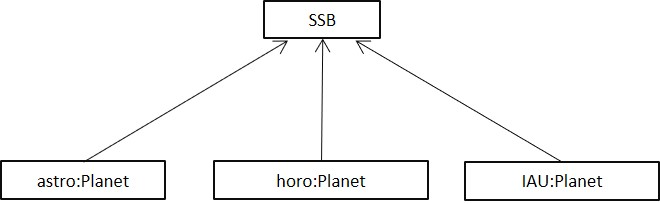
\includegraphics[width=5.0in]{SWWOv3/media/ch2/f02-01.jpg}
    \caption{Subclass diagram for different notions of planet.}
    \label{fig:ch2.1}
\end{figure}


\begin{figure}
    \centering
    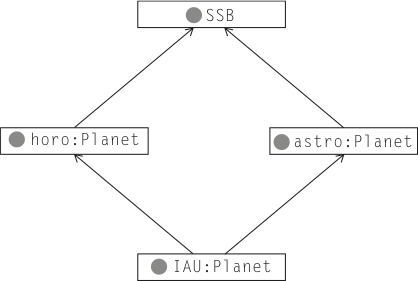
\includegraphics[width=5.0in]{SWWOv3/media/ch2/f02-02.jpg}
    \caption{More detailed relationships between various notions of planet.}
    \label{fig:ch2.2}
\end{figure}


\subsection{Variation and layers}

Classes and subclasses are a fine way to organize variation when there
is a simple, known relationship between the modeled entities and it is
possible to determine a clear ordering of classes that describes these
relationships. In a Web setting, however, this usually is not the case.
Each contributor can have something new to say that may fit in with
previous statements in a wide variety of ways. How can we accommodate
variation of sources if we can't structure the entities they are
describing into a class model?

The Semantic Web provides an elegant solution to this problem. The basic
idea is that any model can be built up from contributions from multiple
sources. One way of thinking about this is to consider a model to be
described in layers. Each layer comes from a different source. The
entire model is the combination of all the layers, viewed as a single,
unified whole.

Let's have a look at how this could work in the case of Pluto. Figure~\ref{fig:ch2.3} 
illustrates how different communities could assert varying
information about Pluto. In part (a) of the figure, we see some
information about Pluto that is common among astrologers---namely, that
Pluto signifies rebirth and regeneration and that the preferred symbol
for referring to Pluto is the glyph indicated. Part (b) shows some
information that is of concern to astronomers, including the composition
of the body Pluto and their preferred symbol. How can this variation be
accommodated in a web of information? The simplest way is to simply
merge the two models into a single one that includes all the information
from each model, as shown in part (c).

\begin{figure}
    \centering
    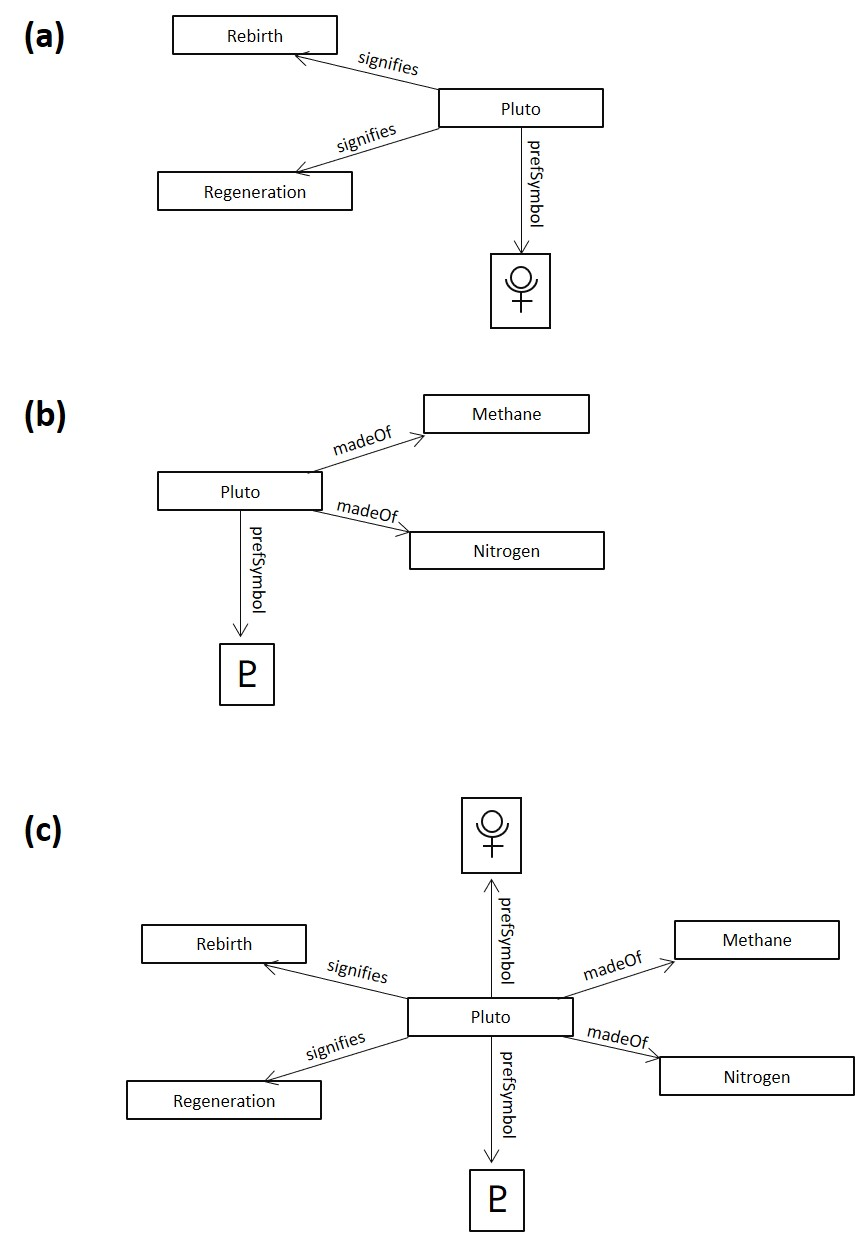
\includegraphics[width=5.0in]{SWWOv3/media/ch2/f02-03abc.jpg}
    \caption{Layers of modeled information about Pluto.}
    \label{fig:ch2.3}
\end{figure}

Merging models in this way is a conceptually simple thing to do, but how
does it cope with variability? In the first place, it copes in the
simplest way possible: It allows the astrologers and the astronomers to
both have their say about Pluto (remember the AAA slogan!). For any
party that is interested in both of these things (perhaps someone
looking for a spiritual significance for elements?), the information can
be viewed as a single, unified whole.

But merging models in this way has a drawback as well. In Figure~\ref{fig:ch2.3}(c),
there are two distinct glyphs, each claiming to be the ``preferred''
symbol for Pluto. This brings up issues of consistency of viewpoints. On
the face of it, this appears to be an inconsistency because, from its
name, we might expect that there can be exactly one preferred symbol
(prefSymbol) for any solar system body. But how can a machine know that?
For a machine, the name prefSymbol can't be treated any differently from
any other label---for instance, madeOf or signifies. In such a context,
how can we even tell that this is an inconsistency? After all, we don't
think it is an inconsistency that Pluto can be composed of more than one
chemical compound or that it can signify more than one spiritual theme.
Do we have to describe this in a natural language commentary on the
model?

Detailed answers to questions like these are exactly the reason why we
need to publish models on the Semantic Web. When two (or more!)
viewpoints come together in a web of knowledge, there will typically be
overlap, disagreement, and confusion before there is synergy,
cooperation, and collaboration. If the infrastructure of the Web is to
help us to find our way through the wild stage of information sharing,
an informal notion of how things fit together, or should fit together,
will not suffice. It is easy enough to say that we have an intuition
that states there is something special about prefSymbol that makes it
different from madeOf or signifies. If we can inform our infra-
structure about this distinction in a sufficiently formal way, then it
can, for instance, detect discrepancies of this sort and, in some cases,
even resolve them.

This is the essence of modeling in the Semantic Web: providing an
infrastructure where not only can anyone say anything about any topic
but the infrastructure can help a community work through the resulting
chaos. A model can provide a framework (like classes and subclasses) for
representing and organizing commonality and variability of viewpoints
when they are known. But in advance of such an organization, a model can
provide a framework for describing what sorts of things we can say about
something. We might not agree on the symbol for Pluto, but we can agree
that it should have just one preferred symbol.

\section{Expressivity in Modeling}

There is a trade-off when we model, and although anyone can say anything
about any topic, not everyone will want to say certain things. There are
those who are interested in saying details about individual entities,
like the preferred symbol for Pluto or the themes in life that it
signifies. Others (like that IAU) are interested in talking about
categories, what belongs in a category, and how you can tell the
difference. Still others (like lexicographers, information architects,
and librarians) want to talk about the rules for specifying information,
such as whether there can be more than one preferred label for any
entity. All of these people have contributions to make to the web of
knowledge, but the kinds of contributions they make are very different,
and they need different tools. This difference is one of \emph{level of
expressivity}.

The idea of different levels of expressivity is as well known in the
history of collaborative human knowledge as modeling itself. Take as an
example the development of models of a water molecule, as

\begin{figure}
    \centering
    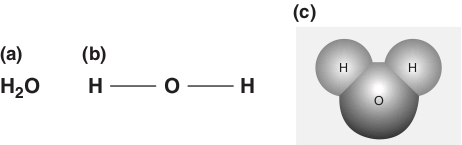
\includegraphics[width=5.0in]{media/ch2/f02-04ac-9780123859655.jpg}
    \caption{Different expressivity of models of a water molecule.}
    \label{fig:ch2.4}
\end{figure}


shown in Figure~\ref{fig:ch2.4}. In part (a), we see a model of the water molecule
in terms of the elements that make up the molecule and how many of each
is present -- namely, two hydrogen atoms and one oxygen atom. This model
expresses important information about the molecule, and it can be used
to answer a number of basic questions about water, such as calculating
the mass of the molecule (given the masses of its component atoms) and
what components would have to be present to be able to construct water
from constituent parts.

In Figure~\ref{fig:ch2.4}(b), we see a model with more expressivity. Not only does
this model identify the components of water and their proportions, but
it also shows how they are connected in the chemical structure of the
molecule. The oxygen molecule is connected to each of the hydrogen
molecules, which are not (directly) connected to one another at all.
This model is somewhat more expressive than the model in part (a); it
can answer further questions about the molecule. From (b), it is clear
that when the water molecule breaks down into smaller molecules, it can
break into single hydrogen atoms (H) or into oxygen-hydrogen ions (OH)
but not into double-hydrogen atoms (H2) without some recombination of
components after the initial decomposition.

Finally, the model shown in Figure~\ref{fig:ch2.4}(c) is more expressive still in
that it shows not only the chemical structure of the molecule but also
the physical structure. The fact that the oxygen atom is somewhat larger
than the hydrogen atoms is shown in this model. Even the angle between
the two hydrogen atoms as bound to the oxygen atom is shown. This
information is useful for working out the geometry of combinations of
water molecules, as is the case, for instance, in the crystalline
structure of ice.

Just because one model is more expressive than another does not make it
superior; different expressive modeling frameworks are different tools
for different purposes. The chemical formula for water is simpler to
determine than the more expressive, but more complex, models, and it is
useful for resolving a wide variety of questions about chemistry. In
fact, most chemistry textbooks go for quite a while working only from
the chemical formulas without having to resort to more structural models
until the course covers advanced topics.

The Semantic Web provides a number of modeling languages that differ in
their level of expressivity; that is, they constitute different tools
that allow different people to express different sorts of information.
In the rest of this book, we will cover these modeling languages in
detail. The Semantic Web standards are organized so that each language
level builds on the one before so the languages themselves are layered.
The following are the languages of the Semantic Web from least
expressive to most expressive.

\emph{RDF} \emph{--} \emph{The Resource Description Framework}. This is
the basic framework that the rest of the Semantic Web is based on. RDF
provides a mechanism for allowing anyone to make a basic statement about
anything and layering these statements into a single model. Figure 2.3
shows the basic capability of merging models in RDF. The work on RDF
started in 1997 and it has been a recommendation from the W3C since
1999, updated in 2004 and in 2014 with RDF 1.1.

\emph{SHACL} \emph{-- The Shapes Constraint Language.} SHACL is a language
based on the intuition that we expect data to be in a certain form, or \emph{shape}.
SHACL allows a modeler to represent the expected shape of a data description. These shapes can be
used to validate data or to present a form to a human user to fill out to supply data.
Unlike the other Semantic Web modeling languages, which are designed based on the Open World Assumption, SHACL works with the Closed World Assumption; if data is not included in   a description, then it is considered to be missing. 
SHACL is one of the newest modeling languages in the semantic web stack, and became a
W3C Recommendation in 2017. 

\emph{RDFS} \emph{-- The RDF Schema language.} RDFS is a language with
the expressivity to describe the basic notions of commonality and
variability familiar from object languages and other class systems---
namely classes, subclasses, and properties. Figures~\ref{fig:ch2.1} and \ref{fig:ch2.2}
illustrated the capabilities of RDFS. RDFS was drafted in 1999 and
became a W3C recommendation in 2004.

\emph{RDFS-Plus}. RDFS-Plus is a subset of OWL that is more expressive
than RDFS but without the complexity of OWL. There is no standard in
progress for RDFS-Plus, but there is a growing awareness that something
between RDFS and OWL could be industrially relevant. We have selected a
particular subset of OWL functionality to present the capabilities of
OWL incrementally. RDFS-Plus includes enough expressivity to describe
how certain properties can be used and how they relate to one another.
RDFS-Plus is expressive enough to show the utility of certain constructs
beyond RDFS, but it lacks the complexity that makes OWL daunting to many
beginning modelers. The issue of uniqueness of the preferred symbol is
an example of the expressivity of RDFS-Plus.

\emph{OWL} \emph{-- the Web Ontology Language}. OWL brings the
expressivity of logic to the Semantic Web. It allows modelers to express
detailed constraints between classes, entities, and properties. OWL was
adopted as a recommendation by the W3C in 2004, with a second version
adopted in 2009.

\section{SUMMARY}

The Semantic Web, just like the hypertext web that preceded it, is based
on some radical notions of information sharing. These ideas \emph{--}
the AAA slogan, the open world assumption, and nonunique naming
\emph{--} provide for an environment in which information sharing can
thrive and a network effect of knowledge synergy is possible. But this
style of information gathering creates a chaotic landscape rife with
confusion, disagreement, and conflict. How can the infrastructure of the
Web support the development from this chaotic state to one characterized
by information sharing, cooperation, and collaboration?

The answer to this question lies in modeling. Modeling is the process of
organizing information for community use. Modeling supports this in
three ways: It provides a framework for human communication, it provides
a means for explaining conclusions, and it provides a structure for
managing varying viewpoints. In the context of the Semantic Web,
modeling is an ongoing process. At any point in time, some knowledge
will be well structured and understood, and these structures can be
represented in the Semantic Web modeling language. At the same time,
other knowledge will still be in the chaotic, discordant stage, where
everyone is expressing himself differently. And typically, as different
people provide their own opinions about any topic under the sun, the Web
will simultaneously contain organized and unorganized knowledge about
the very same topic. The modeling activity is the activity of distilling
communal knowledge out of a chaotic mess of information. This was nicely
illustrated in the Pluto example.

The next several chapters of the book introduce each of the modeling
languages of the Semantic

Web and illustrate how they approach the challenges of modeling in a
Semantic Web context. For each

modeling language \emph{--} RDF, RDFS, and OWL \emph{--} we will
describe the technical details of how the language works, with specific
examples ``in the wild'' of the standard in use.

\subsection{Fundamental concepts}

The following fundamental concepts were introduced in this chapter.

\emph{\textbf{Modeling}} \emph{--} Making sense of unorganized
information.

\emph{\textbf{Formality/Informality}} \emph{--} The degree to which the
meaning of a modeling language is given independent of the particular
speaker or audience.

\emph{\textbf{Commonality and Variability}} \emph{--} When describing a
set of things, some of them will have some things in common
(commonality), and some will have important differences (variability).
Managing commonality and variability is a fundamental aspect of modeling
in general, and of Semantic Web models in particular.

\emph{\textbf{Expressivity}} \emph{--} The ability of a modeling
language to describe certain aspects of the world. More expressive
modeling language can express a wider variety of statements about the
model. Modeling languages of the Semantic Web---RDF, RDFS, and
OWL---differ in their levels of expressivity.
